% Created 2022-09-20 Tue 11:28
% Intended LaTeX compiler: pdflatex
\documentclass[11pt]{article}
\usepackage[mathletters]{ucs}
\usepackage{hyperref}
\usepackage{amsmath}
\usepackage{listings}
\usepackage{xcolor}
\usepackage{graphicx}
\definecolor{codegreen}{rgb}{0,0.6,0}
\definecolor{codegray}{rgb}{0.5,0.5,0.5}
\definecolor{codepurple}{rgb}{0.58,0,0.82}
\definecolor{backcolour}{rgb}{0.95,0.95,0.92}
\lstdefinestyle{mystyle}{
backgroundcolor=\color{backcolour},
commentstyle=\color{codegreen},
keywordstyle=\color{magenta},
numberstyle=\tiny\color{codegray},
stringstyle=\color{codepurple},
basicstyle=\ttfamily\footnotesize,
breakatwhitespace=false,
breaklines=true,
captionpos=b,
keepspaces=true,
numbers=left,
numbersep=5pt,
showspaces=false,
showstringspaces=false,
showtabs=false,
tabsize=2
}
\lstset{style=mystyle, language=Python}
\author{Habib Ghaffari}
\date{2022-09-19 Mon}
\title{Tutorial \#1 - What You Need to Know About the Tutorials}
\hypersetup{
 pdfauthor={Habib Ghaffari},
 pdftitle={Tutorial \#1 - What You Need to Know About the Tutorials},
 pdfkeywords={},
 pdfsubject={},
 pdfcreator={Emacs 28.1 (Org mode 9.5.2)}, 
 pdflang={English}}
\begin{document}

\maketitle
\tableofcontents




\section{Introduction}
\label{sec:org977a8da}

My name is \texttt{Habib Ghaffari Hadigheh}. It is a mouthful name so you can simply
call me \texttt{Habib} whenever you see me on campus. I am a fourth-year Ph.D.
student under the supervision of Dr. Christopher Anand. My main area of
research is Machine Learning (ML), Operations Research (Or) and Signal
Processing. You can find information about how to contact me via my website at
the following address \href{https://ghhabib.me}{Here}.

ghaffh1

Today we are going to learn how to work with the course's website, how to
install \texttt{Python} interpreter, and how to write our first program in python to
make sure our interpreter is working properly. I am also going to introduce an
IDE helps you to do coding much easier. If we have time I am also
going to start working on a very simple language and try to write some
programs based on it and see how our example program going to be evaluated.

\section{Objectives of this tutorial}
\label{sec:orga2bcc62}

At the end of this session you should be able to :

\begin{itemize}
\item Learn to work with the website.
\item Install the python interpreter in different operating systems.
\item Install IDE for coding.
\item Write our first \texttt{Python} program.
\item Try to define a very simple language.
\end{itemize}

\subsection{Learn How to Work With the Course's website}
\label{cp2:s1}
Here is the website address:

\href{http://www.cas.mcmaster.ca/\~franek/courses/cs3mi3/}{http://www.cas.mcmaster.ca/\textasciitilde{}franek/courses/cs3mi3/}

On this website, you can find the course outline, a page for
announcements and a link to \href{http://www.cas.mcmaster.ca/\~franek/courses/cs3mi3/login/startlogin.cgi}{sign in} to your page. You should receive an
email around a week ago with your username and password.

\begin{figure}[!ht]
\centering

\includegraphics[width=0.8\textwidth]{./figures/1.png}
\caption{\label{fig1}Course Page}
\end{figure}

\begin{figure}[!ht]
\centering
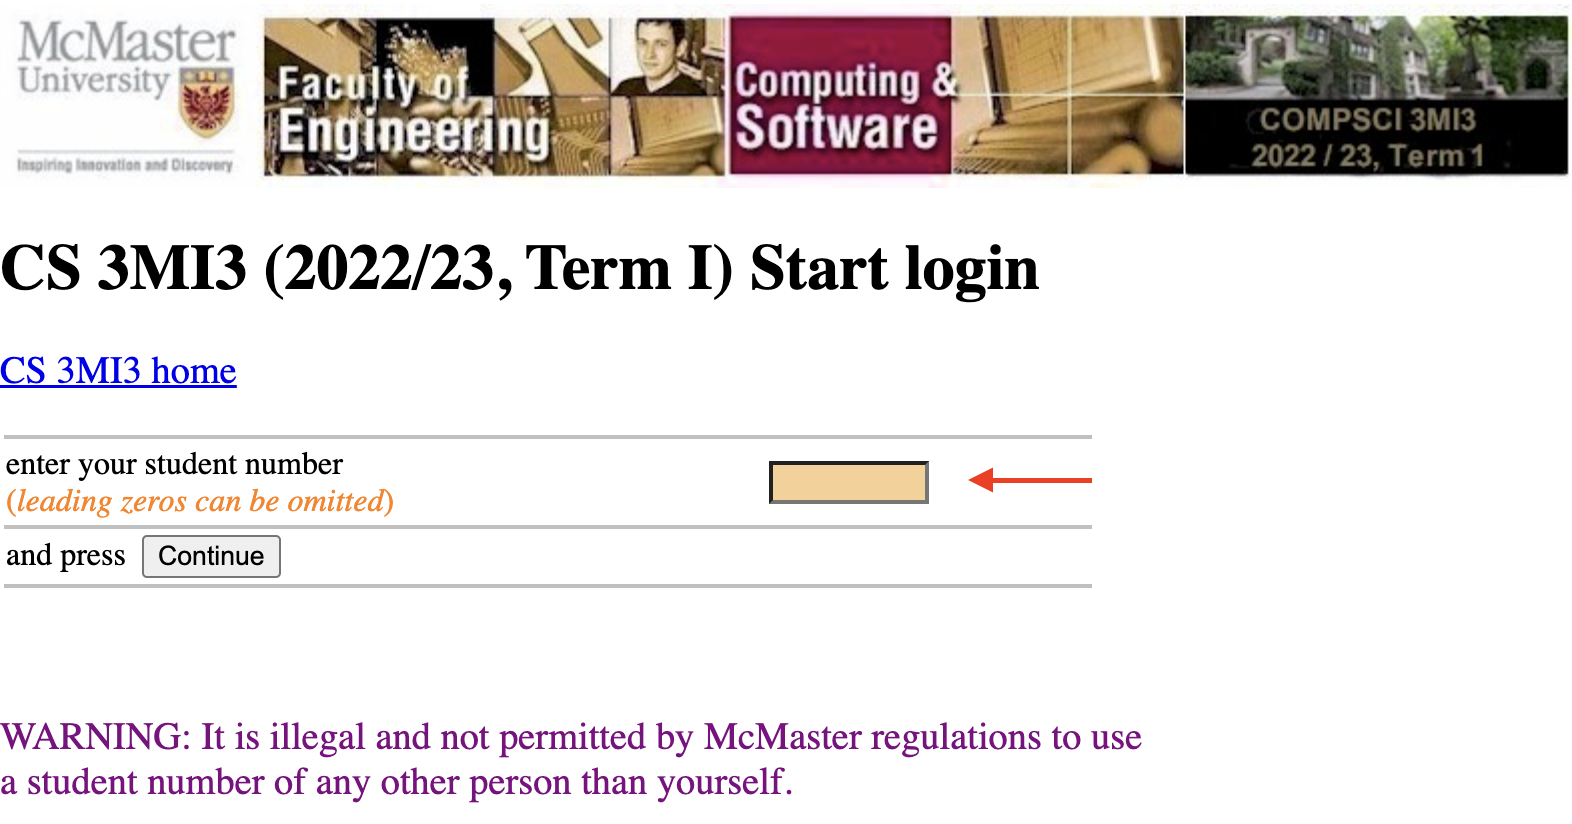
\includegraphics[width=0.8\textwidth]{./figures/2.png}
\caption{\label{fig2}Login Page (Put your user name)}
\end{figure}

\begin{figure}[!ht]
\centering
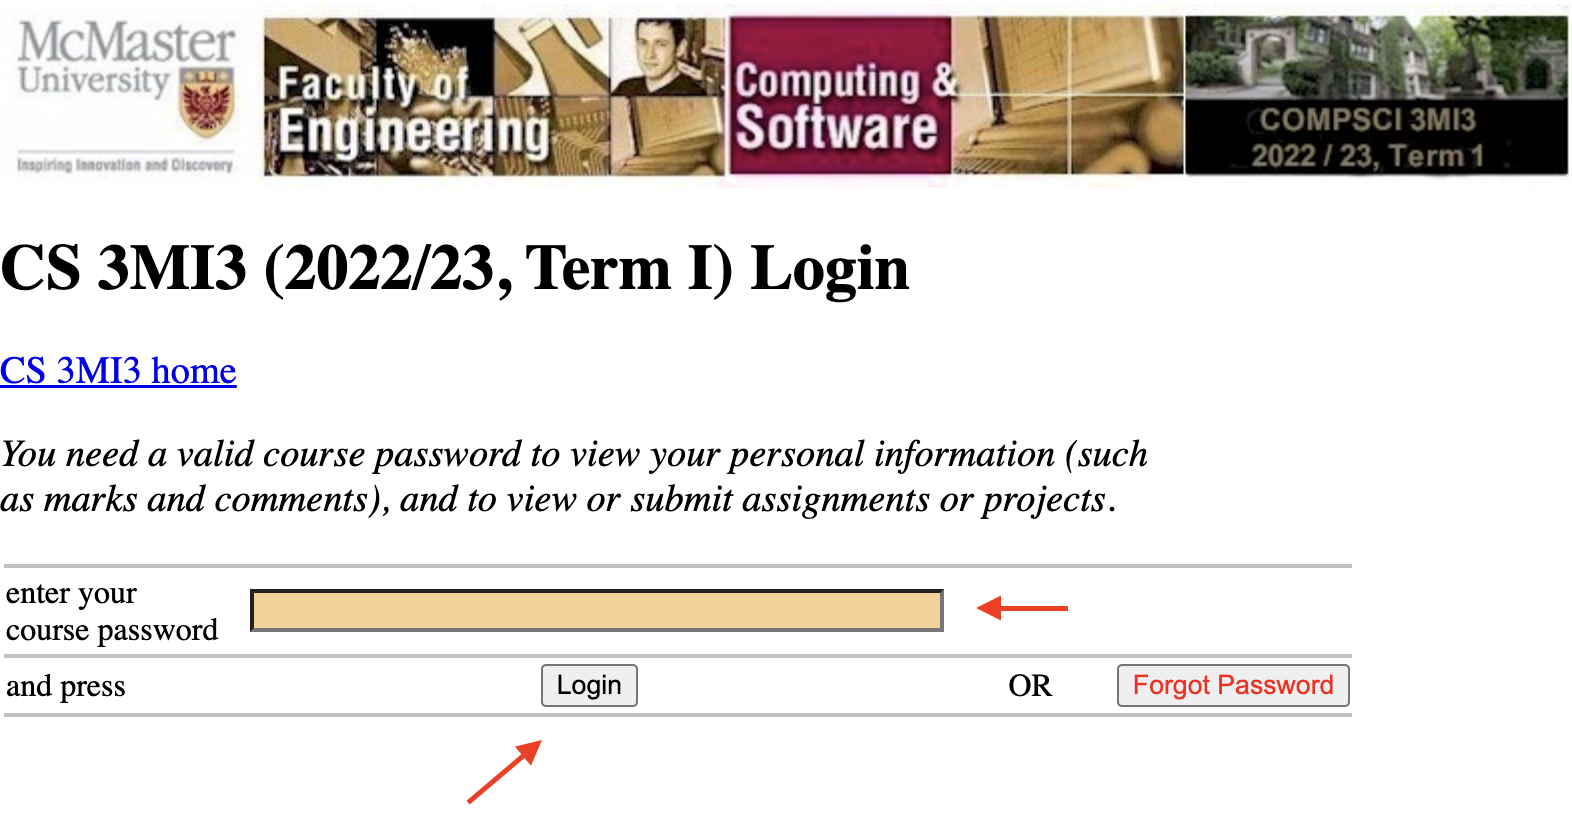
\includegraphics[width=0.8\textwidth]{./figures/3.png}
\caption{\label{fig3}Login Page (Type your password)}
\end{figure}

\subsubsection{Resolve your problems}
\label{sec:orgd5fa0df}

\begin{itemize}
\item As TAs, we do not have any office hours, but we are available via email and you
can schedule online/in-person meetings with any of us by emailing us.

\item Problems with marking may happen in any course. If you think there is any
problem with your marking or the comments/feedback you received is unclear,
please contact me. I will figure out who marked your assignment/exam and make
sure they provide you with more clarification about your mark. If you are
still not satisfied I will ask another TA to mark your submission again. The
final step would be for either me or Dr. Franek to look at your solution and
make the final decision.
\end{itemize}

\subsection{How to Install \texttt{Python} Interpreter:}
\label{sec:orga9c7938}

\subsubsection{Windows}
\label{sec:org70dac2b}

There are a few methods to install \texttt{Python} interpreter on your machine. The
straightforward method is to use \texttt{Python} website.

\url{https://www.python.org/}

Another method is to use \texttt{Chocolatey}. You can install \texttt{Chocolatey} using the
following link:

\url{https://chocolatey.org/install}

Then you can simply use the following link to install a version of \texttt{Pthon} on
your machine:

\url{https://community.chocolatey.org/packages/python/3.9.1}

Another method is to use \texttt{Anaconda}:

\url{https://www.anaconda.com/}


\subsubsection{Mac OS}
\label{sec:org178f8bb}

Mac OS should have an in-built \texttt{Python} version pre-installed on the Machine.
However, you can easily install a version based on your preferences:

The straightforward method again is to use the website:

\url{https://www.python.org/downloads/macos/}

But the most preferable method is to use \texttt{Homebrew}. You can install \texttt{HomeBrew}
on your machine using the following link:

\url{https://brew.sh/}

The next step is to use the following instruction to install any version of
python you want:

\begin{verbatim}
brew install python
\end{verbatim}


\subsubsection{Linux (Ubuntu)}
\label{sec:orgad4c9a1}

Installing \texttt{Python} on a Linux (Ubuntu) machine is very easy. Just type the
following command in your terminal

\begin{verbatim}
sudo apt-get install python
\end{verbatim}


\subsection{IDE for \texttt{Python} Coding}
\label{sec:orgcf35967}

You can use almost any editor to implement python programs. However, the best
well-known IDE is \texttt{Pycharm}:

\url{https://www.jetbrains.com/pycharm/}


\subsection{Implement Our First \texttt{Python} Program}
\label{sec:orga7b2e5c}

Let's implement our \texttt{Hello World} program in \texttt{Python}.

\begin{verbatim}
print("Hello World!!")
\end{verbatim}


\subsection{Simple Language}
\label{sec:org814992f}


Let's have a look at the \texttt{BNF} as you know it:

\begin{verbatim}
 <postal-address> ::= <name-part> <street-address> <zip-part>

      <name-part> ::= <personal-part> <last-name> <opt-suffix-part> <EOL> | <personal-part> <name-part>

  <personal-part> ::= <initial> "." | <first-name>

 <street-address> ::= <house-num> <street-name> <opt-apt-num> <EOL>

       <zip-part> ::= <town-name> "," <state-code> <ZIP-code> <EOL>

<opt-suffix-part> ::= "Sr." | "Jr." | <roman-numeral> | ""
    <opt-apt-num> ::= <apt-num> | ""
\end{verbatim}


This translates into English as:

\begin{itemize}
\item A postal address consists of a name-part, followed by a street-address part,
followed by a zip-code part.
\item A name-part consists of either: a personal-part followed by a last name
followed by an optional suffix (Jr., Sr., or dynastic number) and end-of-line,
or a personal part followed by a name part (this rule illustrates the use of
recursion in BNFs, covering the case of people who use multiple first and
middle names and initials).
\item A personal-part consists of either a first name or an initial followed by a
dot.
\item A street address consists of a house number, followed by a street name,
followed by an optional apartment specifier, followed by an end-of-line.
\item A zip-part consists of a town-name, followed by a comma, followed by a state
code, followed by a ZIP-code followed by an end-of-line.
\item An opt-suffix-part consists of a suffix, such as "Sr.", "Jr." or a
roman-numeral, or an empty string (i.e. nothing).
\item An opt-apt-num consists of an apartment number or an empty string (i.e.
nothing).
\end{itemize}


The language we are going to define contains just a handful of syntactic forms:
the boolean constants \texttt{true} and \texttt{false}, conditional expressions, the numeric
constant 0, the arithmetic operators \texttt{succ} (successor) and \texttt{pred} (predecessor),
and a testing operation \texttt{iszero} that returns \texttt{true} when it is applied to \texttt{0} and
\texttt{false} when it is applied to some other number.

\begin{verbatim}
<t> ::=                      Term
    T                        Constant True
    F                        Constant False
    0                        Zero
    if t then t else t       Conditional Expression
    succ t                   Successor
    pred t                   Predecessor
    iszero t                 Zero Test
\end{verbatim}

A program in the present language is just a term built from the forms given by
the grammar above. Here are some examples of programs, along with the results of
evaluating them:

\begin{verbatim}
if (F) then 0 else (succ 0);
> succ 0

iszero (pred (succ 0));
> T
\end{verbatim}


What is the evaluation result of the following programs?

\begin{verbatim}
> if (succ 0) then 0 else pred (succ (succ (0)));
> if 0 then T else F;
> iszero (T);
\end{verbatim}


Exercise:

\begin{itemize}
\item How could we evaluate the above expression?
\end{itemize}


Now let's define the above language using \texttt{Haskell} programming language:


\begin{verbatim}
data term =
     T -- True Constant
    |F -- False Constant
    |Zero -- Zero Constant
    |Succ term -- Successor
    |Pred term -- Predecessor
    |IfThenElse term term term -- Conditional Expression
    |IsZero term -- Zero Test
\end{verbatim}

Exercise:

\begin{itemize}
\item How could we define the language rules using \texttt{Haskell}?

\item Is it possible to define this language in \texttt{Python}? If yes then how?
\end{itemize}
\end{document}